\chapter{Machine Learning Architectures for Tone Reservation}
\label{ch:dl_tr}

One of the techniques discussed in the first phase of this project is Tone Reservation (TR) \cite{original_tr}. It is a distortionless technique, with no effect on the integrity of the data being sent, and only a slight reduction in the data rate since we reserve some of the subcarriers to form a new peak-cancelling signal. While the classical Tone Reservation algorithm successfully mitigates PAPR, its iterative gradient-descent approach suffers from slow convergenec and sub-optimal peak cancellation. This chaper introduces the application of Deep Learning (DL) to the TR framework, exploring various neural network architectures designed to learn and optimize the peak-canceling signal generation process.

\section{Tone Reservation (TR) Principles in the Context of ML}
Before detailing the specific neural network implementations, it is necessary to re-contextualize the Tone Reservation technique for machine learning environments. The fundamental principle of TR remains the same: a set of reserved subcarriers, $\mathcal{R}$, which carry no user data, are used to generate a time-domain compensating signal, $c[n]$. The transmitted time-domain signal is expressed as:
\begin{equation*}
    x_{tx}[n] = x_{data}[n] + c[n]
\end{equation*} \cite{original_tr}
In classical TR, $c[n]$ is generated iteratively by shifting and scaling a predefined time-domain kernel $p[n]$. In the context of Machine Learning, the neural networks are tasked with observing $x_{data}[n]$ and directly outputting or optimizing the scaling factors and parameters required to generate the optimal $c[n]$ in a fraction of the time required by classical methods.

\section{Feedforward Neural Network Approaches (TRNet)}
The first investigated architecture follows the purely data-driven paradigm. The Tone Reservation Network (TRNet) utilizes a Feedforward Neural Network (FFNN) to adaptively generate the peak-canceling signal, completely bypassing the sub-optimal iterative gradient search of classical TR \cite{trnet}.

\subsection{System Architecture and Data Preprocessing}

\begin{figure}[H]
    \centering
    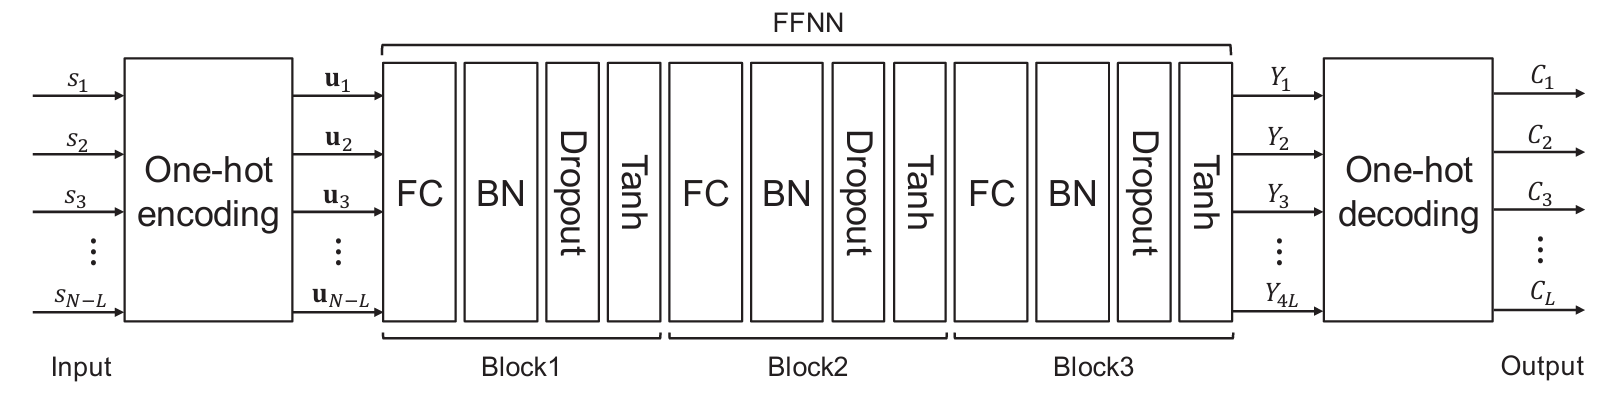
\includegraphics[width=0.9\textwidth]{Figures/DL_TR/trnet_block_diagram.png}
    \caption{Block diagram of the TRNet architecture, illustrating the feedforward neural network structure for peak-canceling signal generation.}
    \label{fig:trnet_architecture}
\end{figure}
The TRNet is deployed exclusively at the transmitter. The neural network consists of five layers connected in tandem: one input layer, three hidden layers, and one output layer \cite{trnet}. Because standard neural networks cannot process complex baseband signals natively, the TRNet architecture employs a specific data preprocessing step utilizing one-hot encoding. For a 4-QAM modulation scheme, each 2-bit symbol is mapped to a 4-dimensional real-valued unit vector (e.g., $00 \leftrightarrow [1,0,0,0]$). This mapping not only circumvents the complex number limitation but also forces the data into a sparse representation that is highly conducive to machine learning optimization \cite{trnet}. At the output, the network decodes every four consecutive real-valued bits back into a complex 4-QAM reserved symbol.

\subsection{Hidden Layer Cascade Blocks}
To effectively map the input signal to the optimal peak-canceling vector, the three hidden layers are structured into identical cascade blocks. Each block is composed of:
\begin{itemize}
    \item \textbf{Fully Connected (FC) Layer:} Extracts the nonlinear characteristics of the signal through matrix multiplication and feature space transformation.
    \item \textbf{Batch Normalization (BN) Layer:} Normalizes the output of the FC layer to avoid vanishing gradients, dynamically adjusting the distribution during training to significantly accelerate convergence.
    \item \textbf{Dropout Layer:} Implements a regularization scheme that randomly zeroes out half of the feature detectors in each training batch (satisfying a Bernoulli distribution). This drastically reduces interactions among dependent feature detectors, preventing the model from overfitting to the training data.
    \item \textbf{Activation Function:} Utilizes the hyperbolic tangent (tanh) function. Since the BN layer limits data to the $[-1, 1]$ interval where tanh closely resembles the identity function ($y=x$), this choice improves overall training efficiency.
\end{itemize}

\subsection{Training Characteristics}
The TRNet is trained to minimize a custom loss function that strictly calculates the PAPR of the composite transmitted signal, expressed as $LOSS = PAPR\{Q(X+C)\}$, where $Q$ is the IFFT matrix \cite{trnet}. The network parameters are optimized offline using the Adaptive Moment Estimation (Adam) algorithm. Due to its architecture, TRNet requires only a small number of datasets for the model to converge quickly, providing excellent robustness and allowing for rapid retraining if waveform parameters change \cite{trnet}.

\section{Model-Driven Deep Learning Tone Reservation (DL-TR)}
\subsection{Model-Based Deep Learning}

\subsubsection{Introduction to the Spectrum of Inference}
Traditional signal processing and communications have long relied on classical statistical modeling techniques \cite{modelbased}. These model-based methods utilize mathematical formulations designed from domain knowledge, prior information, and an understanding of the underlying physics. For example, the classical Tone Reservation (TR) gradient algorithm operates entirely on the deterministic mathematical properties of the OFDM signal. While these simple classical models are tractable, understandable, and computationally efficient, they are often sensitive to inaccuracies and fail to capture the nuances of dynamic, high-dimensional complex data.

Conversely, purely data-driven approaches, such as standard Deep Neural Networks (DNNs), use generic, highly-parameterized architectures to map inputs to predictions \cite{modelbased}. These methods, like the TRNet architecture discussed earlier, are model-agnostic and do not rely on analytical approximations. However, they suffer from significant drawbacks when applied to telecommunications: they require massive amounts of training data, demand immense computational resources, and operate as opaque "black boxes" lacking the interpretability and reliability of model-based methods.

\subsection{Bridging the Gap: Model-Based Deep Learning}
To overcome the limitations of both extremes, a hybrid methodology known as Model-Based Deep Learning has emerged as a cornerstone of modern physical layer design \cite{modelbased}. These methods combine principled mathematical models with data-driven systems to benefit from the advantages of both approaches. By exploiting partial domain knowledge through mathematical structures designed for specific problems, these systems can learn effectively from much more limited data.

This hybrid paradigm is systematically divided into two main strategies: \textit{Model-Aided Networks} and \textit{DNN-Aided Inference} \cite{modelbased}.
\begin{itemize}
    \item \textbf{Model-Aided Networks:} These networks implement inference using a DNN, but rather than using a generic architecture, the network is specifically tailored to the scenario by imitating the operation of a model-based algorithm.
    \item \textbf{DNN-Aided Inference:} In this approach, the overall inference is carried out by a traditional model-based method, but specific intermediate computations are augmented or replaced with deep learning tools to overcome missing or inaccurate domain knowledge.
\end{itemize}

\subsection{Deep Unfolding: The Foundation of DL-TR}
The Deep Learning Tone Reservation (DL-TR) architecture implemented in this graduation project is a quintessential example of a \textbf{Model-Aided Network}, specifically utilizing a technique known as \textit{Deep Unfolding} (or Algorithm Unrolling) \cite{dl_tr}. Deep unfolding converts an iterative optimization algorithm into a DNN by designing each layer to resemble a single iteration. Rather than forcing a generic neural network to learn the physics of OFDM peak cancellation from scratch, the architecture's topology is strictly dictated by the mathematical equations of the classical algorithm.

\subsection{Network Structure}
\begin{figure}[H]
    \centering
    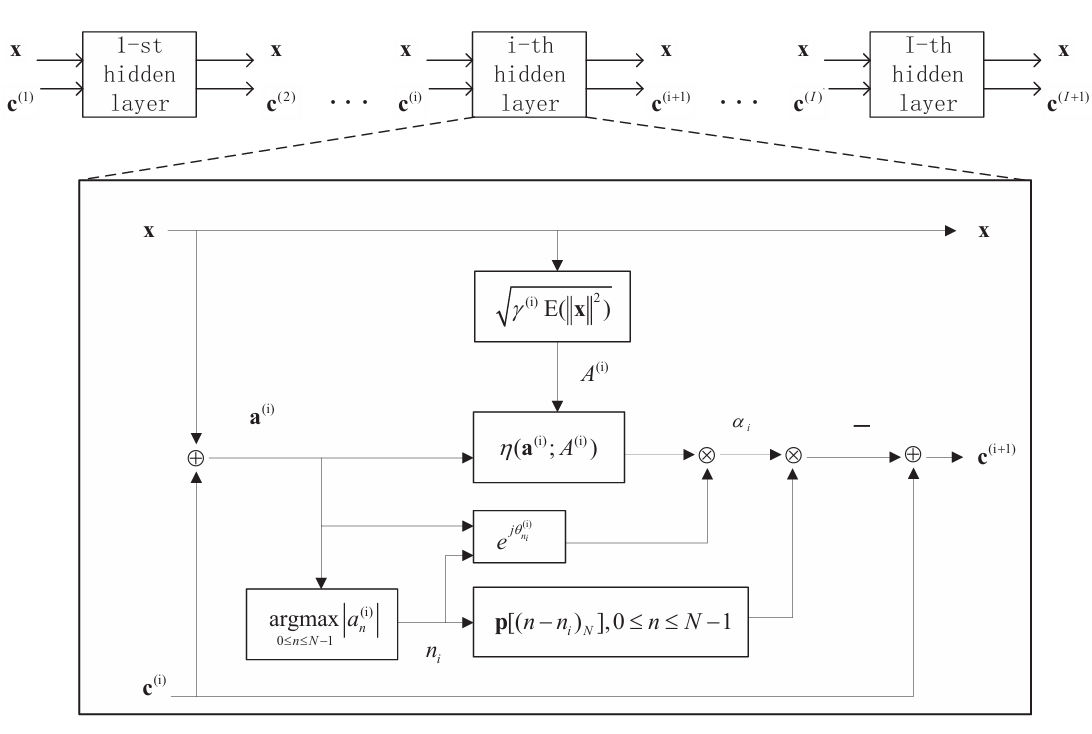
\includegraphics[width=0.70\textwidth]{Figures/DL_TR/DL_TR_block_diagram.png}
    \caption{Network structure of the DL-TR architecture, demonstrating the deep unfolding of the iterative Tone Reservation algorithm into trainable cascade layers.}
    \label{fig:dl_tr_network_structure}
\end{figure}

The application of deep unfolding to the PAPR reduction problem perfectly aligns with the systematic design outline for model-aided networks established in the literature \cite{modelbased}:
\begin{enumerate}
    \item \textbf{Identifying the Iterative Algorithm:} The classical TR gradient-descent optimization is identified as the foundational algorithm suitable for the problem at hand.
    \item \textbf{Fixing the Iterations:} The maximum number of classical iterations in the optimization algorithm is fixed. In the context of DL-TR, this translates to setting exactly $I=8$ hidden layers within the network structure.
    \item \textbf{Imitating Free Parameters in a Trainable Fashion:} Instead of using a static, sub-optimal step size, the architecture is designed to learn the hyperparameters of the objective in each iteration. In DL-TR, this manifests as learning the discrete sequence of clipping ratios, $\theta = \{\gamma_i\}$.
    \item \textbf{End-to-End Training:} The overall unfolded network is trained end-to-end to minimize the loss function. For this system, the unconstrained loss function combining PAPR and the penalty for transmit power increase ($||c||^2$) was optimized via the Adam optimizer.
\end{enumerate}

\subsection{Neural Building Blocks and Extended DL-TR}
The research into the extended DL-TR architecture with trainable time-domain kernel weighting also falls directly under the model-aided networks umbrella. Specifically, it can be viewed through the lens of \textit{Neural Building Blocks} \cite{dl_tr}. This approach acts as a generalization of deep unfolding, representing a model-based algorithm as an interconnection of distinct blocks where each module learns to carry out specific computations. By optimizing both the clipping threshold and the time-domain kernel function simultaneously, the extended DL-TR model utilizes a highly structured, low-rank characteristic. This enables the resulting model to capture known statistical relationships with very few parameters.

\subsection{Advantages Realized in the Implementation}
By evaluating the DL-TR implementation through the lens of model-based deep learning theory, several inherent advantages become apparent that directly contributed to the success of this project phase. Unfolded networks are highly interpretable, possess significantly fewer parameters, and can be trained much more quickly than conventional DNNs \cite{dl_tr}. Because the DL-TR network inherently possesses the mathematical physics of peak reduction, it only needed to learn 8 scalar parameters (the log $\gamma$ values). This allowed the PyTorch implementation to converge in a single epoch using a fraction of the training data required by a black-box autoencoder like TRNet.

Furthermore, a key advantage of deep unfolding over purely model-based optimization is a critical acceleration in inference speed \cite{dl_tr}. By optimizing the layer parameters offline, the DL-TR network achieves superior peak suppression and preserves the Bit Error Rate (BER) over AWGN channels using fewer operational layers than the classical iterative TR algorithm requires to converge. This ultimately proves the immense value of combining rigorous domain knowledge with data-driven tuning.

\subsection{Algorithm Unfolding}
The DL-TR network consists of an input layer, $I$ hidden layers, and a final output layer, where $I$ corresponds to the maximum number of iterations in the classical TR algorithm. At the input layer, the network receives the original time-domain OFDM signal $x$ and initializes the peak-canceling vector to zero ($c^{(1)} = \mathbf{0}$).

\subsection{Forward Pass Dynamics}
Instead of using a static clipping threshold, each unfolded layer $i$ applies a specific, learned clipping ratio $\gamma_i$. The dynamic threshold $A^{(i)}$ is evaluated using the statistical expected power of the original signal $E[||x||^2]$:
\begin{equation*}
    A^{(i)} = \sqrt{\gamma_i E[||x||^2]}
\end{equation*}
The residual magnitude of the peak is calculated and mapped to the phase of the peak to establish the complex scaling factor $\alpha_i$. Finally, the layer generates the updated peak-canceling vector by subtracting a circularly shifted version of the predefined time-domain kernel $p$:
\begin{equation*}
    c^{(i+1)} = c^{(i)} - \alpha_i p[((n-n_i))_N]
\end{equation*}
The network requires only $I$ trainable parameters (the sequence of clipping ratios $\gamma_i$), making it exceptionally lightweight.

\section{Extended Model-Driven TR with Kernel Weighting}
To further push the boundaries of model-driven architectures, an extended DL-TR algorithm incorporating trainable time-domain kernel weights was investigated \cite{extended_dl_tr}. This architecture builds heavily upon the foundational principles of the baseline DL-TR but introduces critical degrees of freedom to suppress residual noise more effectively.

\subsection{Similarities to the Baseline DL-TR}
The extended architecture shares several core philosophies with the baseline DL-TR system implemented in this project:
\begin{itemize}
    \item \textbf{Algorithm Unfolding:} Both networks are explicitly model-driven, unrolling the iterative Tone Reservation scheme into a discrete layer structure rather than using dense, black-box fully connected layers \cite{extended_dl_tr}.
    \item \textbf{Dynamic Thresholding:} Both networks abandon the static, predefined clipping threshold of classical TR. Instead, they utilize the deep learning network to optimize the clipping ratio ($\gamma^{(t)}$) as a trainable parameter in each layer.
    \item \textbf{Loss Function Constraints:} Both networks are trained end-to-end to minimize an unconstrained loss function that actively balances PAPR reduction against a penalty term restricting the average power increase of the peak-canceling signal ($||c||^2$).
\end{itemize}

\subsection{Architectural Differences and Enhancements}
Despite their structural similarities, the extended architecture introduces two major mathematical deviations that significantly alter its peak cancellation dynamics:
\begin{itemize}
    \item \textbf{Simultaneous Multi-Peak Mitigation:} The baseline DL-TR utilizes an $\arg\max$ function to target and cancel only the single highest peak per layer. In contrast, the extended architecture isolates and calculates the largest $L$ peak elements simultaneously in each iteration \cite{extended_dl_tr}.
    \item \textbf{Kernel Weighting Vector:} To cancel these $L$ peaks, the extended network introduces a new trainable scaling vector $\mu_{i}^{(t)}$ \cite{extended_dl_tr}. This parameter dynamically assigns a unique learned weight to the circularly shifted time-domain kernel function for each individual peak, scaling it prior to subtraction.
\end{itemize}

\subsection{Performance Trade-offs}
These architectural enhancements provide a significant boost in performance at the cost of a slight increase in complexity. By actively weighting the kernels and addressing multiple peaks simultaneously, the network effectively mitigates ``peak regrowth''---a common phenomenon where the subtraction of a kernel to cancel one peak inadvertently inflates the signal amplitude at a neighboring index.

This added flexibility means the network possesses more trainable parameters than the baseline DL-TR. For a network configured with $T=5$ layers targeting $L=4$ peaks per layer, the model contains exactly 25 trainable parameters (1 threshold parameter + 4 kernel weight parameters per layer) \cite{extended_dl_tr}. Because the network must sort the signal to find $L$ peaks and compute scaling vectors for each, it exhibits a slightly higher computational complexity (requiring approximately 17,000 Floating-Point Operations, or FLOPs) compared to baseline DL-TR \cite{extended_dl_tr}. Consequently, this model requires marginally more time for both offline training and online inference. However, it remains several orders of magnitude faster and lighter than data-driven architectures like TRNet or PRNet, striking an exceptional balance between parameter efficiency and peak suppression capability.

\section{Simulation Results and Comparative Analysis}

\subsection{Introduction and Simulation Setup}
This chapter presents the simulation results for the various Machine Learning-based Tone Reservation architectures explained above. The simulations were conducted in Python using PyTorch to model both the offline training phases and the online inference phases. The performance of each network is evaluated through Complementary Cumulative Distribution Function (CCDF) curves, Bit Error Rate (BER) analysis, and computational complexity metrics. Furthermore, the results achieved in our simulations are directly compared to the findings reported in the respective reference papers. All simulation results are compared to the work done in \cite{dl_tr}

\subsection{Performance of Model-Driven DL-TR}
The simulations were conducted in Python utilizing PyTorch for the implementation and training of the network. Table \ref{tab:dltr_sim_params} outlines the primary simulation and network parameters utilized throughout the testing phase.

\begin{table}[H]
    \centering
    \caption{DL-TR simulation parameters~\cite{dl_tr}.}
    \label{tab:dltr_sim_params}
    \begin{tabular}{@{} l c l @{}}
        \toprule
        \textbf{Parameter}                   & \textbf{Symbol} & \textbf{Value} \\
        \midrule
        Number of subcarriers                & $N$             & 64             \\
        Number of reserved tones (PRTs)      & $N_t$ / $M$     & 4              \\
        Modulation scheme                    & -               & 4-QAM          \\
        Oversampling factor                  & $U$             & 1              \\
        Training samples                     & $N_s$           & 200,000        \\
        Testing samples                      & $N_{test}$      & 100,000        \\
        Number of hidden layers / iterations & $I$             & 8              \\
        Mini-batch size                      & $D$             & 100            \\
        Learning rate (Adam)                 & $\alpha$        & 0.01           \\
        Power penalty coefficient            & $\lambda$       & 0.1            \\
        Training epochs                      & -               & 1              \\
        Initial clipping ratio               & -               & 4 dB           \\
        \bottomrule
    \end{tabular}
\end{table}

\subsubsection{PAPR Reduction (CCDF)}
The DL-TR network demonstrated vastly superior peak suppression compared to both the Original OFDM signal and the classical TR baseline. The dynamic nature of the learned $\gamma_i$ parameters enabled the network to aggressively target the highest peaks in the early layers while utilizing the final layers to refine the residual noise.

\begin{figure}[H]
    \centering
    \begin{subfigure}[b]{0.48\textwidth}
        \centering
        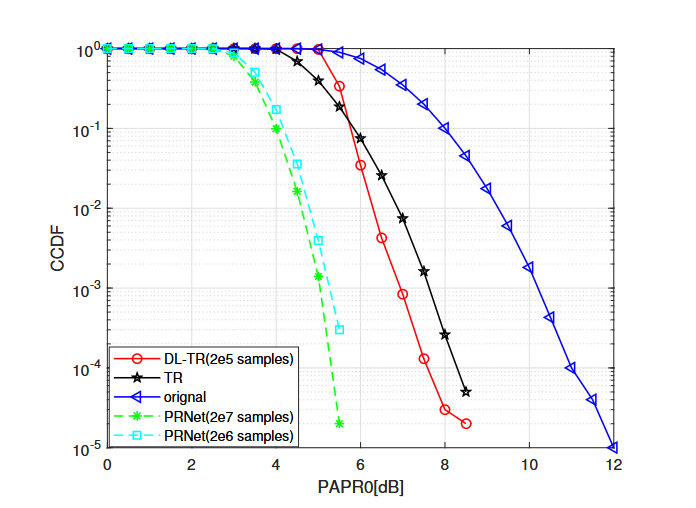
\includegraphics[width=\textwidth]{Figures/DL_TR/dltr_papr_ref.png}
        \caption{Results from the original paper~\cite{dl_tr}}
        \label{fig:dltr_ccdf_paper}
    \end{subfigure}
    \hfill
    \begin{subfigure}[b]{0.48\textwidth}
        \centering
        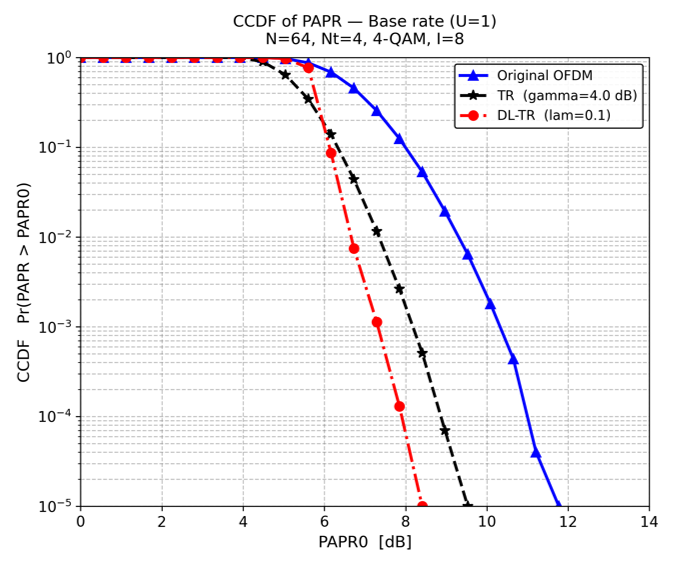
\includegraphics[width=\textwidth]{Figures/DL_TR/dltr_papr_sim.png}
        \caption{Our simulated results}
        \label{fig:dltr_ccdf_sim}
    \end{subfigure}
    \caption{CCDF Comparison of PAPR for Original OFDM, Classical TR, and DL-TR.}
    \label{fig:dltr_ccdf}
\end{figure}

\subsubsection{Bit Error Rate (BER) over AWGN}
To evaluate the true hardware viability of the signal, the transmitted symbols were passed through an Additive White Gaussian Noise (AWGN) channel. Because the DL-TR network actively penalizes the mean-squared power of the peak-canceling vector $||c||^2$ during training via its custom loss function, the resulting signal required significantly less power normalization than classical TR, preserving more energy for the data subcarriers.

\begin{figure}[H]
    \centering
    \begin{subfigure}[b]{0.48\textwidth}
        \centering
        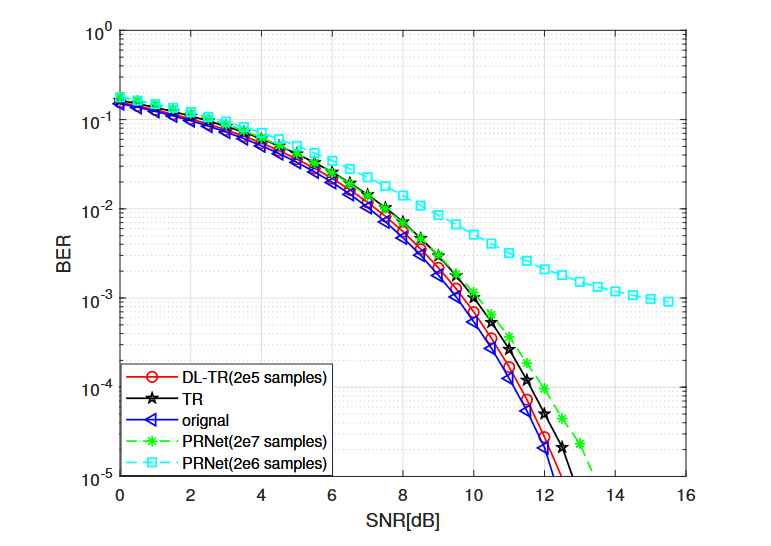
\includegraphics[width=\textwidth]{Figures/DL_TR/dltr_ber_ref.png}
        \caption{Results from the original paper~\cite{dl_tr}}
        \label{fig:dltr_ber_paper}
    \end{subfigure}
    \hfill
    \begin{subfigure}[b]{0.48\textwidth}
        \centering
        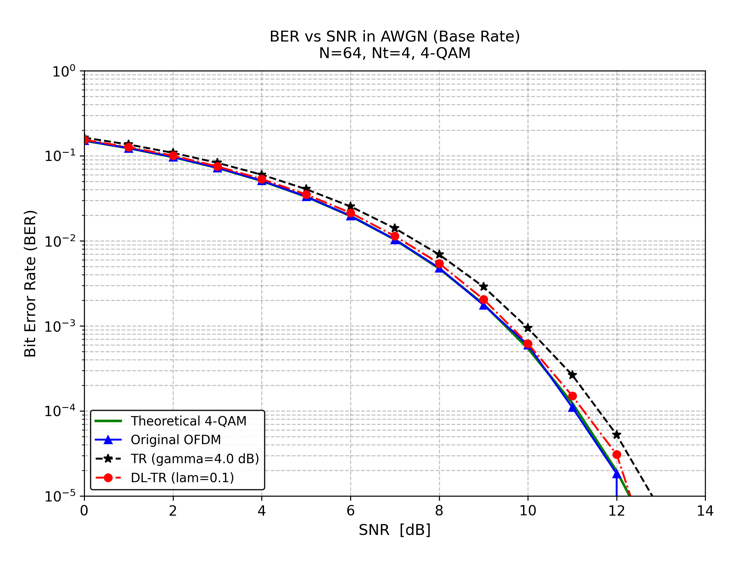
\includegraphics[width=\textwidth]{Figures/DL_TR/dltr_ber_sim.png}
        \caption{Our simulated results}
        \label{fig:dltr_ber_sim}
    \end{subfigure}
    \caption{BER Performance comparison for DL-TR across varying SNR environments.}
    \label{fig:dltr_ber}
\end{figure}

\subsubsection{Effect of the Number of Subcarriers}
To evaluate the scalability and robustness of the DL-TR architecture, simulations were conducted across varying numbers of subcarriers ($N$). As illustrated in Figure \ref{fig:dltr_subcarriers}, while the theoretical PAPR of an OFDM signal naturally increases as the number of subcarriers grows, the DL-TR network maintains its relative suppression efficiency. The unrolled nature of the network allows it to adapt to larger matrix dimensions without requiring a fundamental redesign of the hidden layers.

\begin{figure}[H]
    \centering
    \begin{subfigure}[b]{0.48\textwidth}
        \centering
        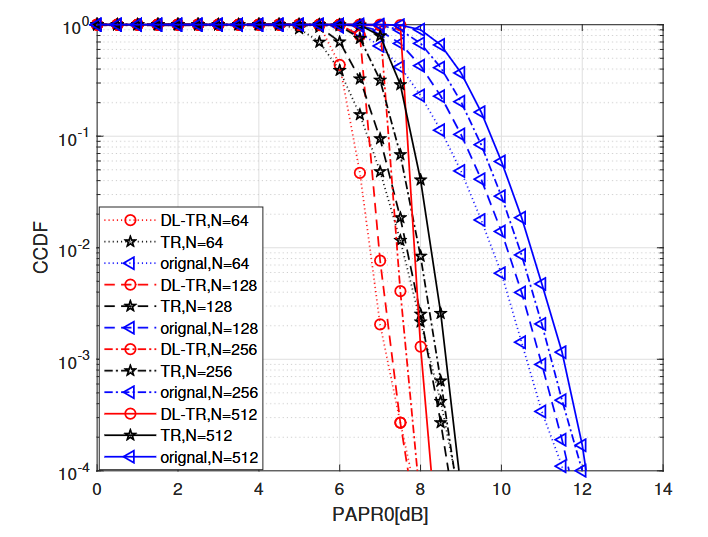
\includegraphics[width=\textwidth]{Figures/DL_TR/dltr_diffN_ref.png}
        \caption{Results from the original paper~\cite{dl_tr}}
        \label{fig:dltr_subcarriers_paper}
    \end{subfigure}
    \hfill
    \begin{subfigure}[b]{0.48\textwidth}
        \centering
        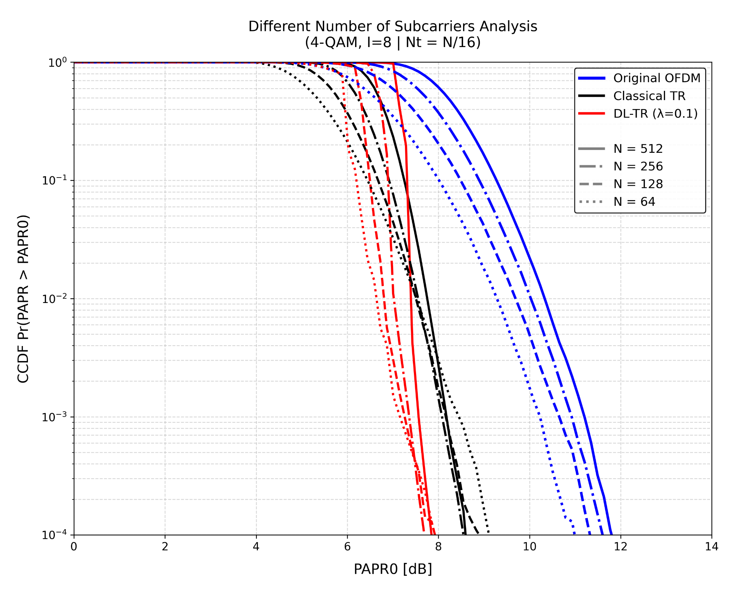
\includegraphics[width=\textwidth]{Figures/DL_TR/dltr_diffN_sim.png}
        \caption{Our simulated results}
        \label{fig:dltr_subcarriers_sim}
    \end{subfigure}
    \caption{Effect of varying the number of subcarriers ($N$) on PAPR reduction.}
    \label{fig:dltr_subcarriers}
\end{figure}

\subsubsection{Runtime and Complexity Comparison}
A crucial advantage of model-driven architectures over classical iterative algorithms is their online inference speed. While the DL-TR network requires an upfront computational investment during the offline training phase, its online execution is highly optimized. As shown in Table \ref{tab:dltr_runtime}, the DL-TR processes symbols significantly faster than classical TR, with around a 3.9 times speedup from the Classical TR. This is because the classical approach must perform dynamic threshold calculations and gradient searches individually for every single symbol, whereas DL-TR applies pre-calculated, optimal $\gamma_i$ tensors via highly parallelized matrix operations.

\begin{table}[H]
    \centering
    \caption{Execution time comparison between Classical TR and DL-TR.}
    \label{tab:dltr_runtime}
    \begin{tabular}{@{} l c c c @{}}
        \toprule
        \textbf{Algorithm}   & \textbf{Training time}  & \textbf{Inference time} & \begin{tabular}{@{}c@{}}\textbf{Average time} \\ \textbf{per symbol}\end{tabular} \\
        \midrule
        Classical TR ($I=8$) & N/A (0 s)               & $\sim$ 1.228 s          & 24.6 $\mu s/sym$                                                                  \\
        DL-TR ($I=8$)        & $\sim$ 15.2 s (1 Epoch) & $\sim$ 0.315 s          & 6.3 $\mu s/sym$                                                                   \\
        \bottomrule
    \end{tabular}
\end{table}

\subsubsection{Effect of Initial Clipping Ratios}
The convergence speed and final PAPR suppression capability of the DL-TR network are influenced by the initialization of the clipping parameters ($\gamma_{init}$) before training commences. Figure \ref{fig:dltr_gamma} compares the network's performance when initialized with different $\gamma_{init}$ values. If the initial ratio is set too high, the early layers fail to identify and clip enough peaks. Conversely, initializing with a value that is too low causes the network to generate an overly aggressive peak-canceling signal, which increases the average transmit power and incurs a heavier loss penalty. The simulations confirm that initializing the learnable parameters near the optimal classical TR clipping ratio provides the best convergence trajectory. The table \ref{tab:sim_params2} shows the parameters of the simulation used to show this effect on the CCDF curve.

\begin{table}[H]
    \centering
    \caption{DL-TR simulation parameters for clipping ratio effect~\cite{dl_tr}.}
    \label{tab:sim_params2}
    \begin{tabular}{@{} l c l @{}}
        \toprule
        \textbf{Parameter}                   & \textbf{Symbol} & \textbf{Value}           \\
        \midrule
        Number of subcarriers                & $N$             & 512                      \\
        Number of reserved tones (PRTs)      & $N_t$ / $M$     & 32                       \\
        Modulation scheme                    & -               & 16-QAM                   \\
        Oversampling factor                  & $U$             & 1                        \\
        Training samples                     & $N_s$           & 20,000                   \\
        Testing samples                      & $N_{test}$      & 500,000                  \\
        Number of hidden layers / iterations & $I$             & 8                        \\
        Mini-batch size                      & $D$             & 100                      \\
        Learning rate (Adam)                 & $\alpha$        & 0.01                     \\
        Power penalty coefficient            & $\lambda$       & 0.1                      \\
        Training epochs                      & -               & 10                       \\
        Initial clipping ratio               & -               & Variable                 \\
        Reserved set positions               & -               & Uses results from GA-PRT \\
        \bottomrule
    \end{tabular}
\end{table}

\begin{figure}[H]
    \centering
    \begin{subfigure}[b]{0.48\textwidth}
        \centering
        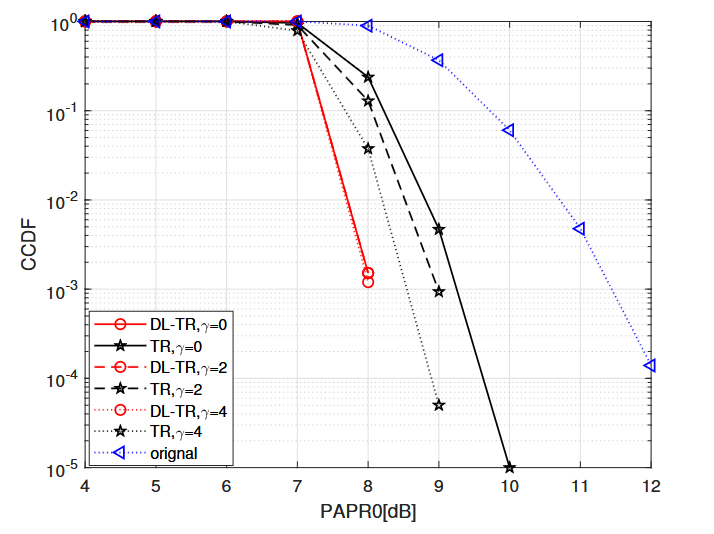
\includegraphics[width=\textwidth]{Figures/DL_TR/dltr_diffG_ref.png}
        \caption{Results from the original paper~\cite{dl_tr}}
        \label{fig:dltr_gamma_paper}
    \end{subfigure}
    \hfill
    \begin{subfigure}[b]{0.48\textwidth}
        \centering
        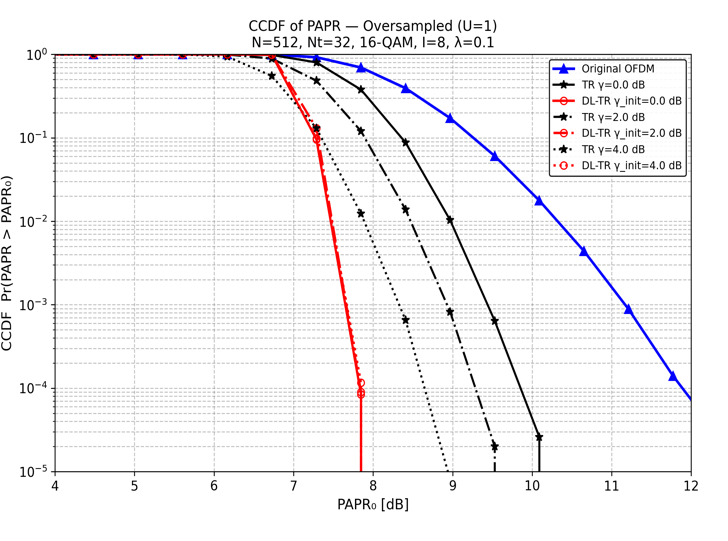
\includegraphics[width=\textwidth]{Figures/DL_TR/dltr_diffG_sim.png}
        \caption{Our simulated results}
        \label{fig:dltr_gamma_sim}
    \end{subfigure}
    \caption{PAPR reduction performance across different initial clipping ratios ($\gamma_{init}$).}
    \label{fig:dltr_gamma}
\end{figure}
